
\chapter{Presentazione risultati}

Nel corso dei precedenti capitoli, sono state fornite le ragioni dietro la scelta dell'architettura neurale NavNet ed è stata descritta l'effettiva struttura implementata in questo lavoro di tesi, è stato discusso il procedimento seguito per la generazione e l'elaborazione del dataset e sono state individuate le misurazioni che, non essendo correlate in maniera significativa alle componenti di spostamento in assi body, possono essere eliminate a monte dell'esecuzione del modello. Terminato, quindi, il lungo e articolato processo di preparazione della rete neurale, non resta che valutarne effettivamente le prestazioni. 

Entrando nel merito dell'analisi svolta, il primo passo consiste nella discussione delle prestazioni della rete neurale nella sua forma "base", così come è stata descritta nel Capitolo 3. Naturalmente, prima di poterne concretamente valutare il comportamento e fare un confronto diretto con i risultati mostrati all'interno del paper di riferimento, occorre determinare gli ultimi due iperparametri a cui ancora non è stato assegnato un valore, ovvero la dimensione di ogni batch e il numero di epoche di addestramento. Successivamente, sulla base dei concetti teorici discussi, è stato svolto uno studio di sensibilità, volto all'individuazione di possibili miglioramenti rispetto alla prima versione. Ovviamente, data l'enorme mole di parametri potenzialmente modificabili, le varianti da valutare sarebbero pressoché infinite. In questa trattazione, pertanto, si è scelto di prendere in considerazione prevalentemente variazioni della dimensionalità del modello, dal punto di vista della hidden size di ogni LSTM, del numero di rami capaci di lavorare in parallelo per giungere alla stima finale e del numero di fully connected layers impiegati per sintetizzare le relazioni individuate dai precedenti layer. Inoltre, è stato valutato l'impatto sulle prestazioni della rete neurale di diverse loss function, potenzialmente molto influenti data la loro importanza all'interno del processo di backpropagation 

Per quanto concerne la metrica principale di valutazione, coerentemente con quanto tipicamente fatto nelle pubblicazioni analizzate nel Capitolo 3, si è scelto di considerare il \emph{Root Mean Squared Error (RMSE)} della posizione, espressa in assi NED locali. Considerando la struttura della suddivisione dei dati utilizzata in questa tesi, le singole traiettorie da valutare in fase di test risultano essere molteplici e, per garantire una maggiore chiarezza espositiva, si è scelto, almeno in fase di confronto preliminare tra le versioni del modello, di considerare unicamente degli indici globali. Nello specifico, oltre alla media dell'RMSE, sono stati utilizzati anche i valori della mediana e del $90^\circ$ e $10^\circ$ percentile. Come sarà evidenziato successivamente, infatti, alcune missioni risultano particolarmente critiche da un punto di vista prestazionale, impattando significativamente sulla media complessiva.  

\section{Valutazione architettura di base}

Come anticipato, il primo passo dell'analisi consiste nella definizione dei due iperparametri mancanti. In merito al primo termine, in particolare, nel Capitolo 2 si erano già identificate delle possibili limitazioni per valori numerici eccessivamente alti o bassi; sulla base di queste indicazioni, quindi, si prendono in considerazione solamente 3 valori: 16 (\textbf{v1.0.01}), 32 (\textbf{v1.0.02}) e 64 (\textbf{v1.0.03}). Per ognuno di questi si addestra un modello differente, sfruttando la struttura base NavNet e un numero di epoche pari a 100, valore puramente indicativo dal momento che quello definitivo non è ancora stato selezionato. I risultati di questo procedimento sono rappresentati graficamente all'interno delle \emph{Figure} \ref{fig:bp_batch} e \ref{fig:rp_sp_batch} e della \emph{Tabella} \ref{tab:v1_batch_results}. 

    \begin{figure}[!htb]
        \centering
        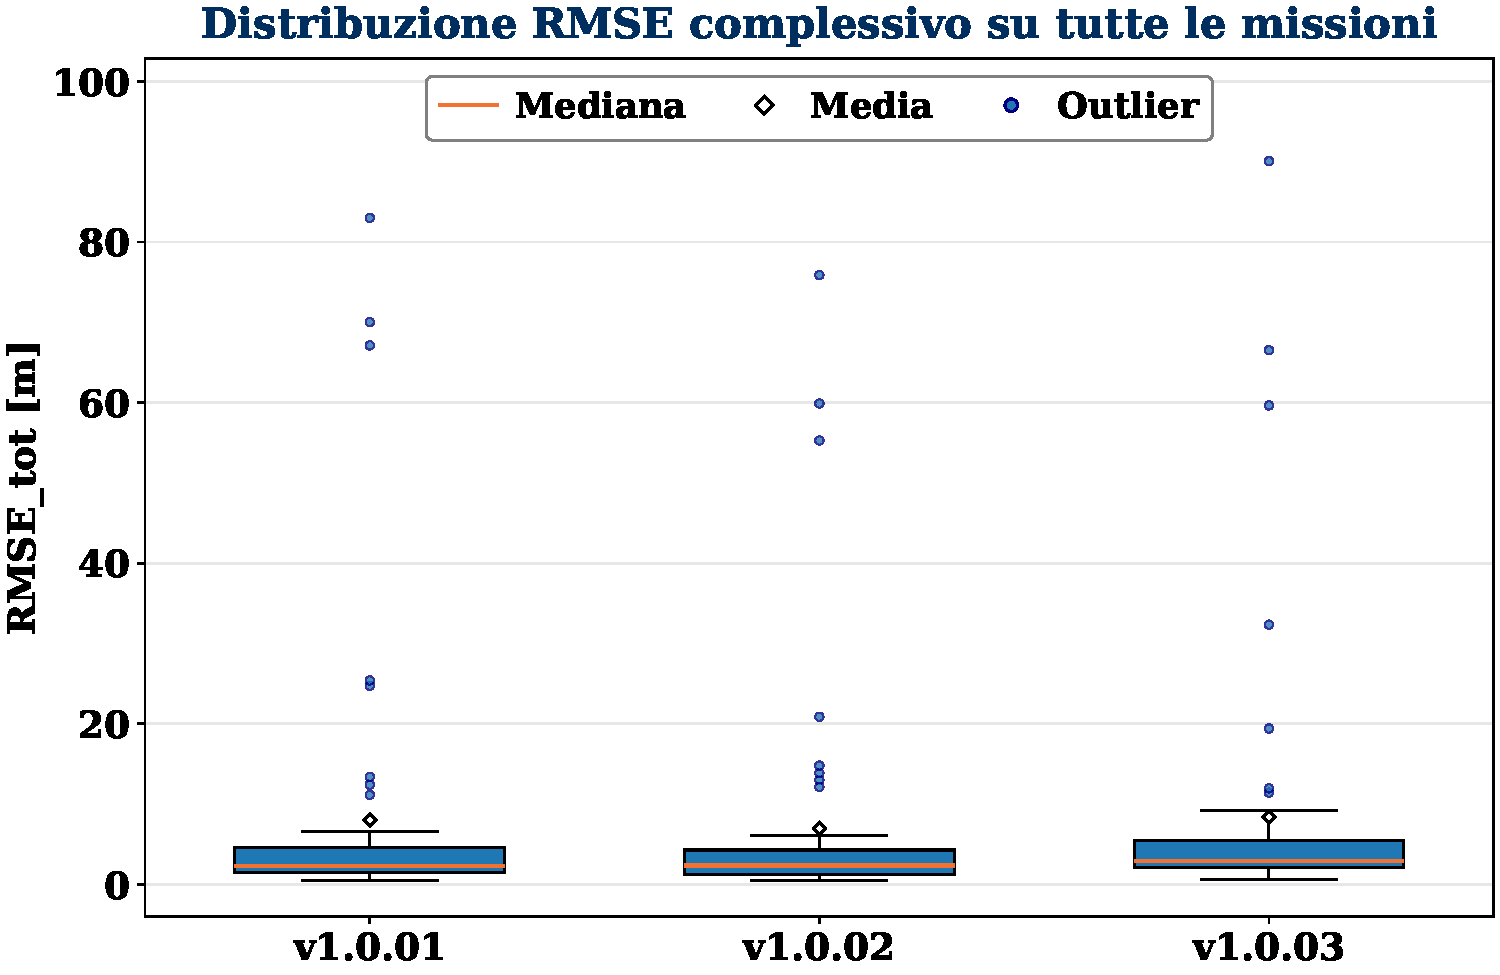
\includegraphics[width=0.8\linewidth]{./images/Risultati/variazioni_batch/Box_plot/RMSE_tot_boxplot_total_missions.pdf}
        \caption{Box plot globale al variare del batch size}
        \label{fig:bp_batch}
    \end{figure}

     \begin{figure}[!htb]

        \centering

        \subfloat[Range plot]{%
                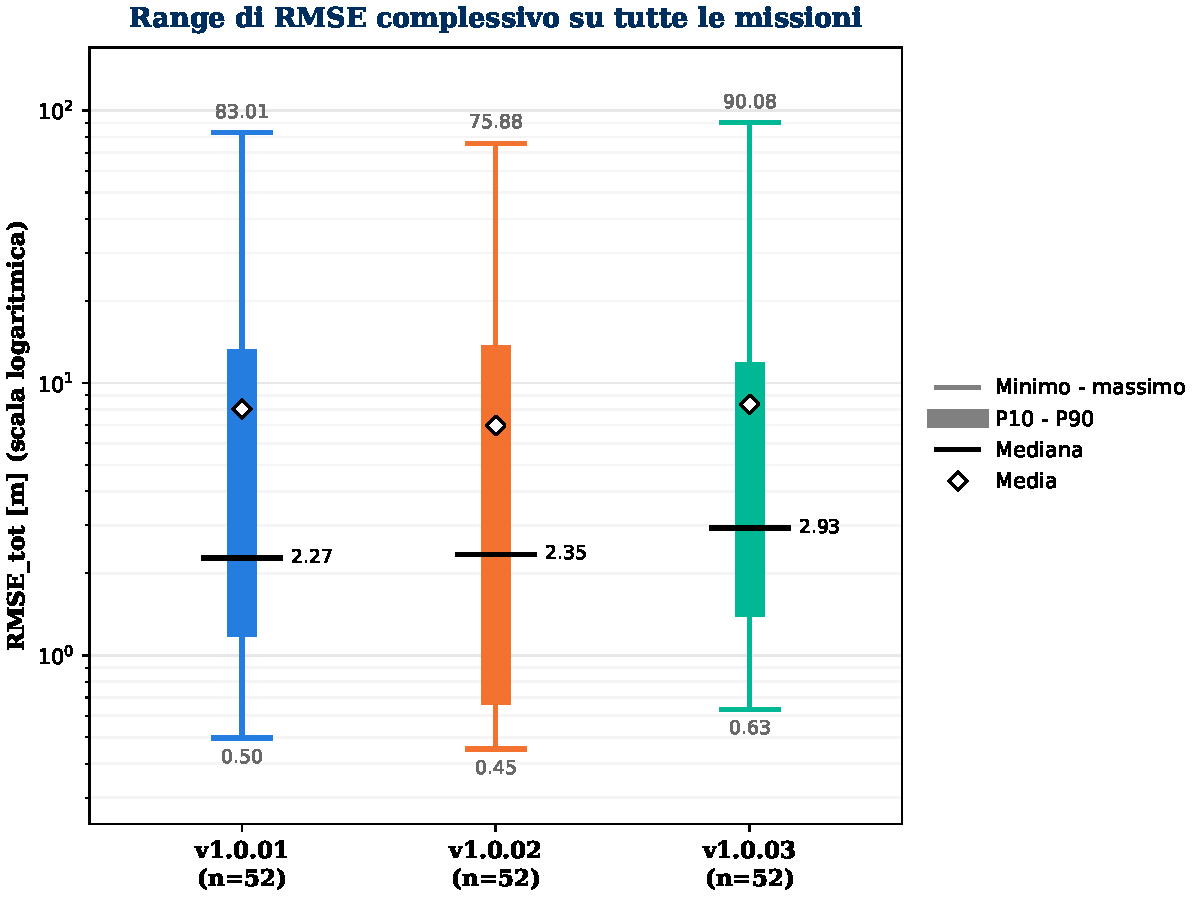
\includegraphics[width=0.50\linewidth]{images/Risultati/variazioni_batch/Range_plot/RMSE_tot_rangeplot_total_missions.pdf}%
                }\hfill
        \subfloat[Scatter plot]{%
                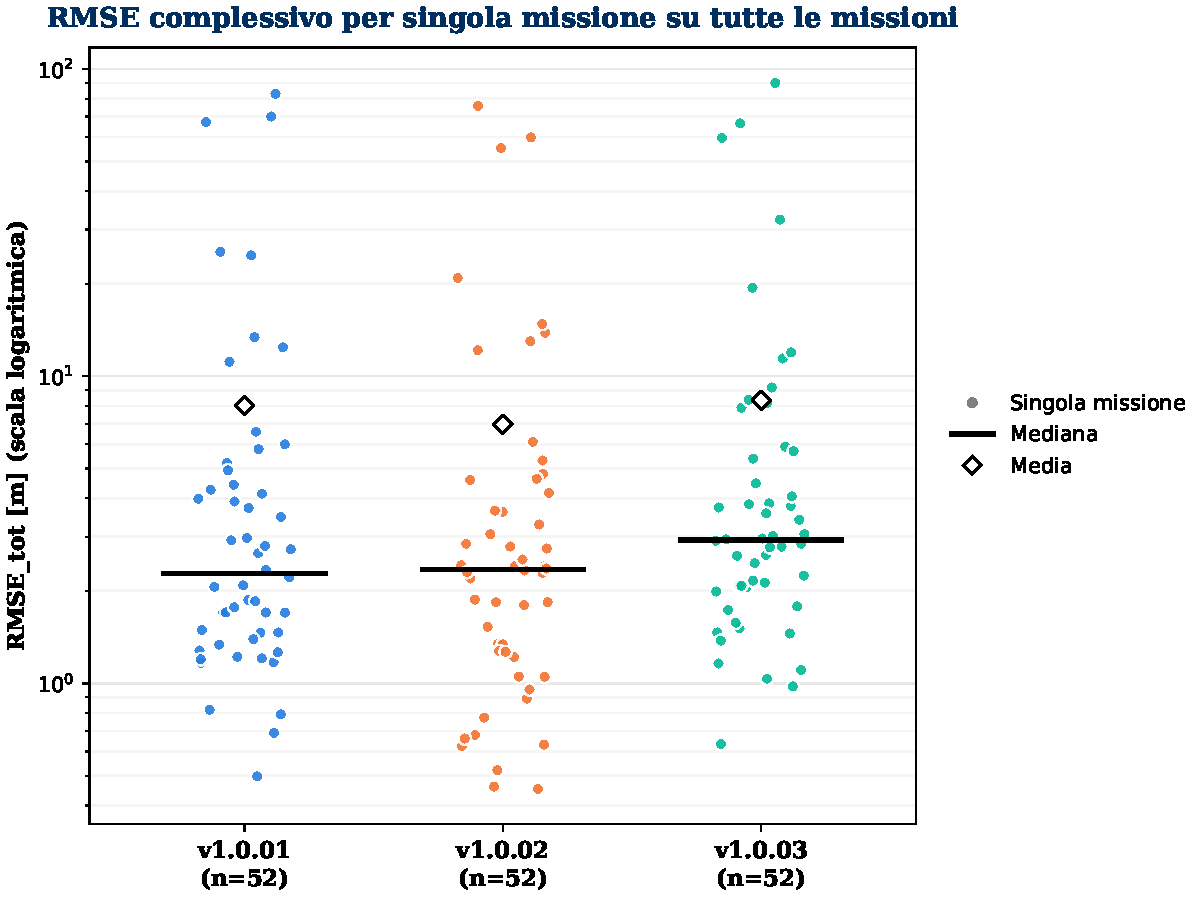
\includegraphics[width=0.49\linewidth]{images/Risultati/variazioni_batch/Strip_plot/RMSE_tot_stripplot_total_missions.pdf}%
                }\\

        \caption{Range plot e scatter plot globali al variare del batch size}
        \label{fig:rp_sp_batch}
                
    \end{figure}

Prima ancora di procedere al confronto relativo tra le versioni proposte, dall'osservazione dei grafici prodotti risalta immediatamente una significativa discrepanza tra i valori di media e mediana dell'RMSE, tratto comune a tutte e tre le versioni. Come verrà discusso più approfonditamente in seguito, un simile comportamento, reiterato anche in tutti i confronti successivi, è dovuto prevalentemente alla presenza di alcune missioni di test particolarmente complesse e, di conseguenza, impegnative per il modello. All'interno dello scatter plot riportato in \emph{Figura} \ref{fig:rp_sp_batch} (a) è possibile osservare una conferma grafica di quanto detto, con circa 8 missioni che risultano caratterizzate da un errore notevolmente superiore alla media. Per comprendere appieno l'entità numerica di questa coda di missioni critiche è, tuttavia, necessario analizzare anche quanto mostrato all'interno del box plot riportato in \emph{Figura} \ref{fig:bp_batch}, dal momento che esso non fa uso di una scala logaritmica per la rappresentazione dei dati. Nel dettaglio, spiccano 3 missioni su tutte, associate ad un RMSE superiore ai 60 metri, con altre 5 caratterizzate da errori compresi tra i 20 e i 40 metri. Tutto ciò è, poi, ulteriormente avvalorato dai dati presentati all'interno della \emph{Tabella} \ref{tab:v1__batch_results}, da cui si evince una netta differenza prestazionale tra le missioni di validazione e quelle di test. Per le prime, infatti, sia la media che la mediana risultano essere molto vicine tra loro, con picchi di errore mai superiori ai 14 metri e, comunque, legati a poche missioni; più nello specifico, poi, si evidenzia un comportamento molto simile tra le prime due versioni, mentre la terza risulta significativamente meno prestazionale, sia dal punto di vista di media e mediana che di dispersione dei valori di errore. Per le sole missioni di test, invece, i valori associati alla media salgono sensibilmente rispetto alle controparti di validazione, a differenza di quelli della mediana che presentano incrementi molto ridotti, pari a circa 3 metri. Nel confronto relativo, in questo caso, emerge una netta superiorità prestazionale della versione basata su una batch\_size pari a 32; questo indica, tendenzialmente, una maggiore capacità di generalizzazione dei dati associata a tale configurazione. Pertanto, nel seguito si considererà questo come il valore di riferimento.    

    \begingroup
        \footnotesize
        \keepXColumns
        \renewcommand{\arraystretch}{1.4}
        \begin{xltabular}{\textwidth}{|>{\centering\arraybackslash}X|>{\centering\arraybackslash}X|>{\centering\arraybackslash}X|>{\centering\arraybackslash}X|>{\centering\arraybackslash}X|>{\centering\arraybackslash}X|}

            \caption{Metriche di valutazione delle versioni di valutazione del batch}
            \label{tab:v1_batch_results} \\
            \hline
            \textbf{Codice versione} & \textbf{Window size} & \textbf{Batch size} & \textbf{Codice versione} & \textbf{Window size} & \textbf{Batch size} \\
            \hline
            \endfirsthead

            \multicolumn{6}{|c|}{{Continua dalla pagina precedente}} \\
            \hline
            \textbf{Codice versione} & \textbf{Window size} & \textbf{Batch size} & \textbf{Codice versione} & \textbf{Window size} & \textbf{Batch size} \\
            \hline
            \endhead

            \hline \multicolumn{6}{|r|}{{Continua nella pagina successiva}} \\ \hline
            \endfoot

            \hline \endlastfoot

            v4.0.01 & 16 & 2 & v4.0.02 & 8 & 4 \\* \cline{1-6}
            v4.0.03 & 32 & 4 & v4.0.04 & 16 & 8 \\* \cline{1-6}
            v4.0.05 & 8 & 2 & v4.0.06 & 4 & 4 \\* \cline{1-6}
            v4.0.07 & 16 & 4 & v4.0.08 & 8 & 8 \\ \hline

        \end{xltabular}
    \endgroup

Per quanto riguarda il secondo parametro, invece, sulla base delle informazioni indirettamente ricavate dalla precedente analisi, si è identificato in $N_{\text{epoche}} = 60$ un compromesso ottimale, capace di garantire i migliori risultati possibili senza necessitare di un tempo di addestramento eccessivo. Quanto appena affermato è corroborato proprio dalle curve di variazione della loss function di training e validazione per ogni epoca, mostrate all'interno della \emph{Figura} \ref{fig:loss_evolution}. In corrispondenza del valore delineato, infatti, si osserva un appiattimento di entrambe le curve, indice di un'interruzione del processo di apprendimento per il raggiungimento di una zona di minimo locale o globale.   

    \begin{figure}[!htb]
        \centering
        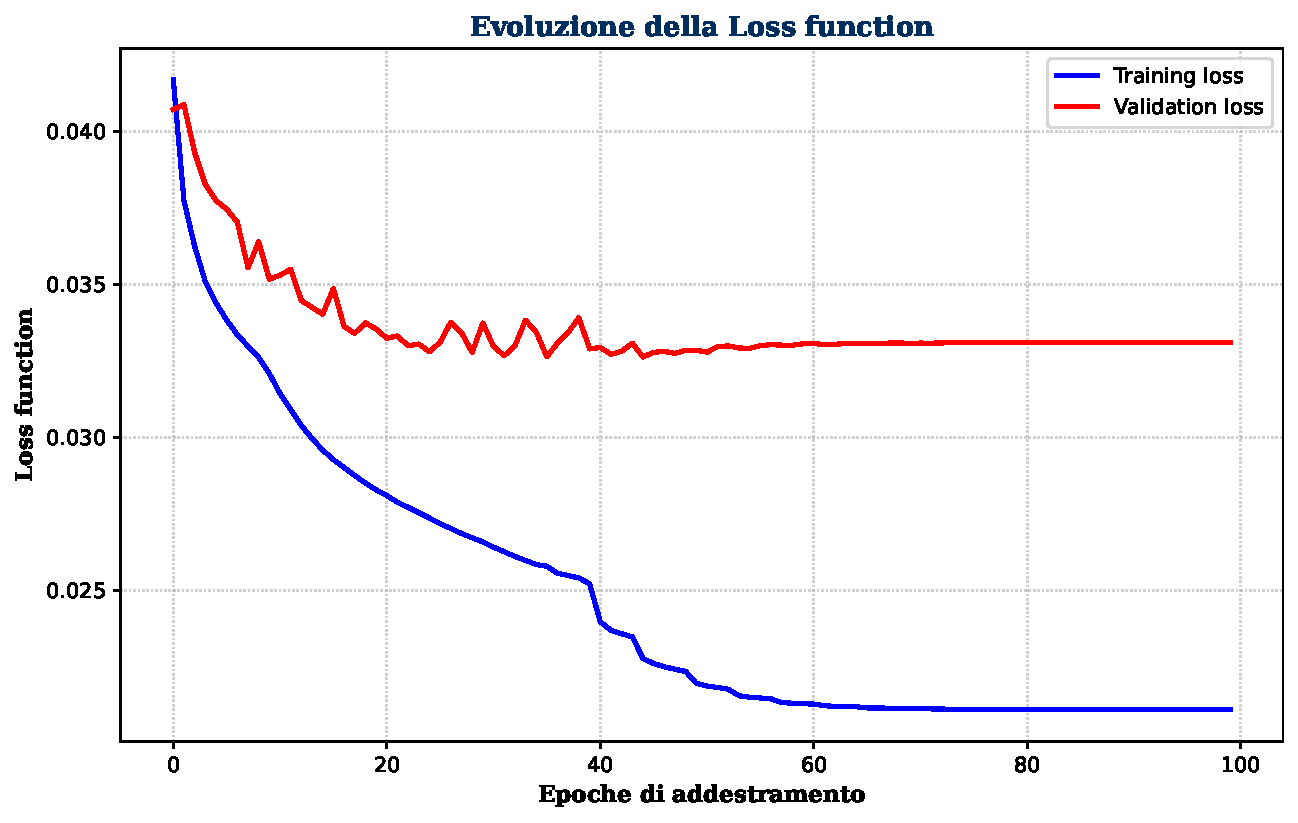
\includegraphics[width=0.6\linewidth]{./images/Risultati/variazioni_batch/Loss_function.pdf}
        \caption{Evoluzione dei valori di loss di training e validazione per epoca}
        \label{fig:loss_evolution}
    \end{figure}

% Si potrebbe aggiungere ma va fatto un nuovo addetramento con 60 epoche e la versione con dataset completo
%La valutazione delle prestazioni della rete neurale con l'utilizzo di 60 epoche di addestramento fornisce, poi, un'ulteriore conferma a supporto della scelta fatta; si osservano, infatti, valori di RMSE medio del tutto identici a quelli mostrati in \emph{Figura} xx. 

Fissati tutti i parametri della rete neurale, occorre svolgere una verifica sperimentale della correttezza delle conclusioni a cui si è giunti a valle dell'analisi di correlazione. Tutti i risultati finora presentati riguardano, infatti, un modello addestrato sul dataset completo, soluzione potenzialmente non ottimale come già si è osservato. Sulla base delle indicazioni fornite all'interno del Capitolo 5, si sono identificati 4 possibili varianti del dataset ridotti:

    \begin{itemize}

        \item \textbf{v1.0.04}: nella prima versione considerata sono state eliminate le sole misurazioni legate alla dinamica verticale dell'AUV, con specifico riferimento a $T_{FV}$, $T_{RV}$, $V_{z_{ref}}$ e $\omega_{y_{\text{ref}}}$. Inoltre, risultando misurazioni quasi mai soggette ad aggiornamento durante la navigazione si scartano $V_{y_{\text{ref}}}$ e $\omega_{x_{\text{ref}}}$ 
        
        \item \textbf{v1.0.05}: nella seconda versione, alle grandezze già scartate si aggiunge il motore laterale posteriore $T_{RL}$. Sebbene esso sia legato allo spostamento lungo l'asse y, presenta una correlazione perfetta con il motore frontale e, pertanto, si può ipotizzare non apporti effettivamente informazioni aggiuntive. 
        
        \item \textbf{v1.0.06}: la terza versione rappresenta sostanzialmente la controparte della precedente, dal momento che viene scartato il motore laterale frontale $T_{FL}$ al posto di quello posteriore. 
        
        \item \textbf{v1.0.07}: quanto fatto finora si basa sull'ipotesi che la dinamica verticale sia completamente slegata dal moto sul piano longitudinale e laterale, non verificabile con certezza. Si sceglie, quindi, di considerare anche una versione che tiene conto dell'influenza del motore verticale posteriore, mentre scarta le informazioni legate al $R_{RL}$; questa scelta è legata, in particolare, alle prestazioni osservate per le due precedenti versioni, con un netto peggioramento nel caso in cui ad essere scartato è il motore $T_{FL}$.
        
    \end{itemize}

    \begin{figure}[!htb]
        \centering
        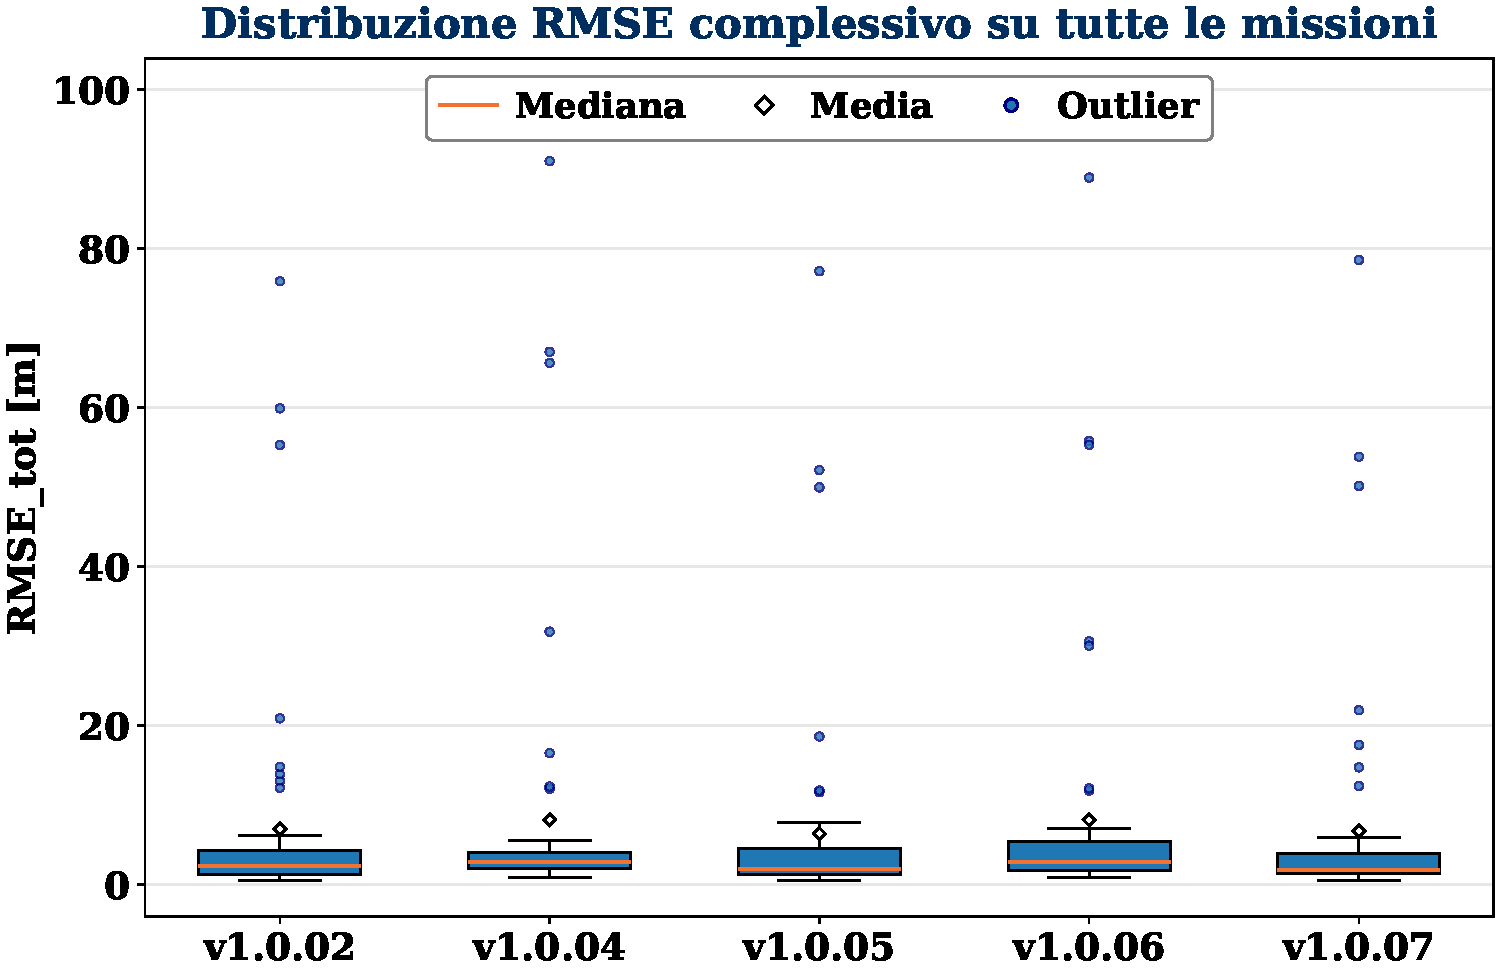
\includegraphics[width=0.8\linewidth]{./images/Risultati/variazioni_dati/Box_plot/RMSE_tot_boxplot_total_missions.pdf}
        \caption{Box plot globale al variare delle features del dataset}
        \label{fig:bp_data}
    \end{figure}

    \begin{figure}[!htb]

        \centering

        \subfloat[Range plot]{%
                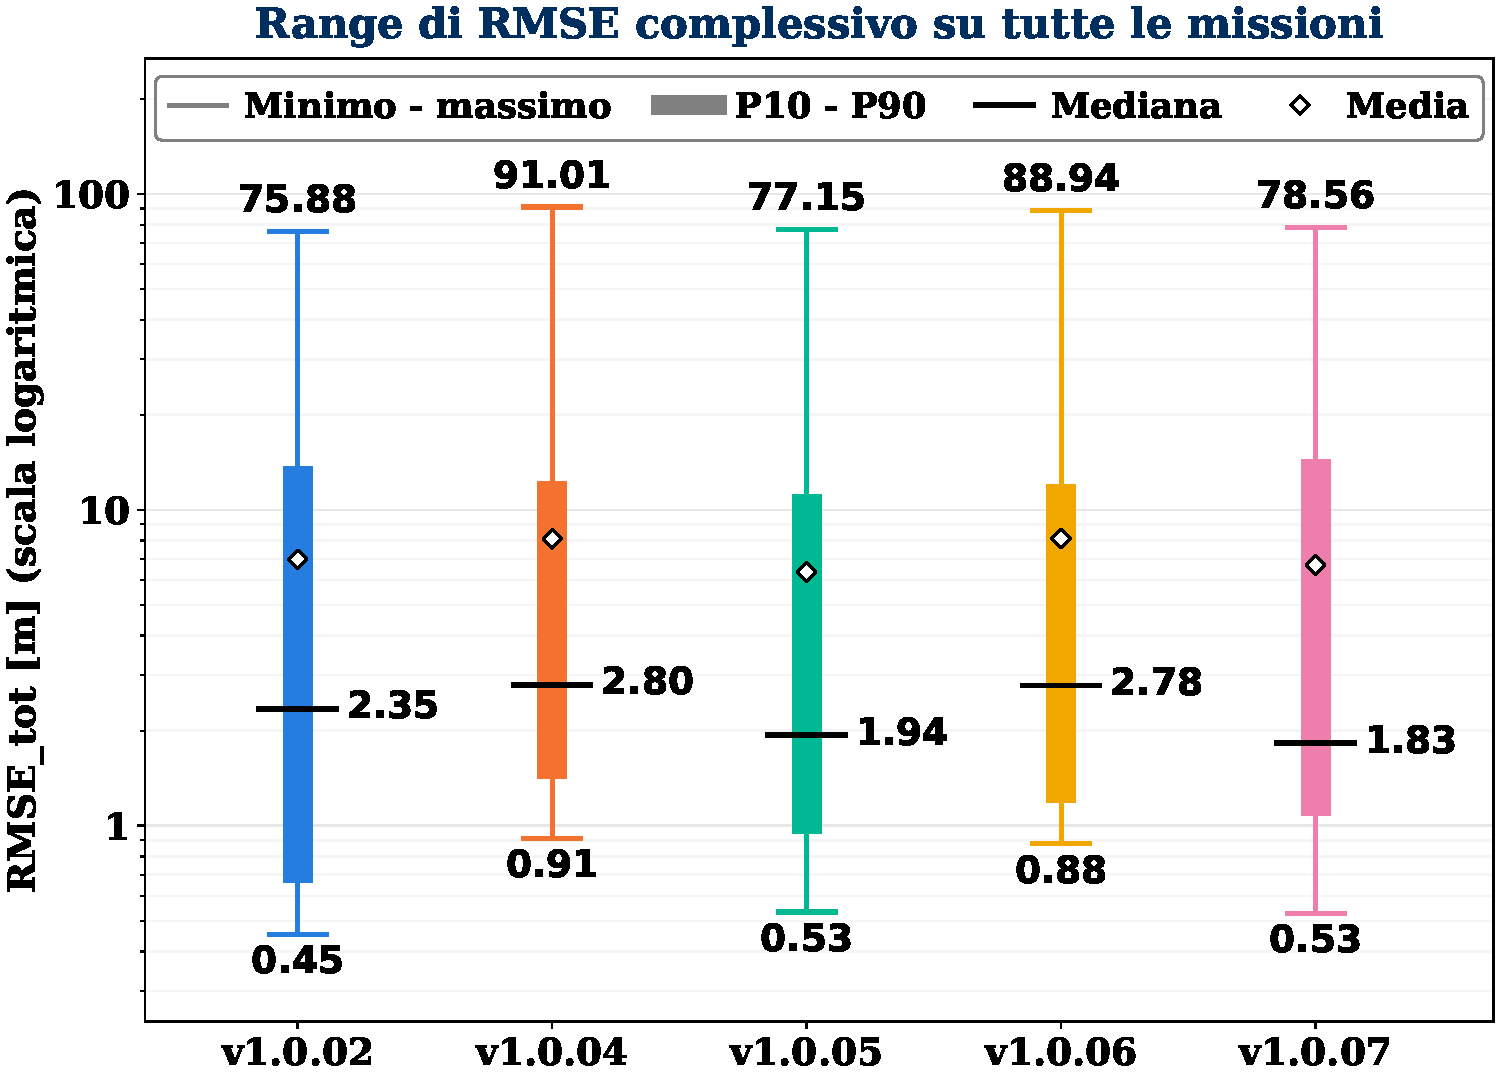
\includegraphics[width=0.50\linewidth]{images/Risultati/variazioni_dati/Range_plot/RMSE_tot_rangeplot_total_missions.pdf}%
                }\hfill
        \subfloat[Scatter plot]{%
                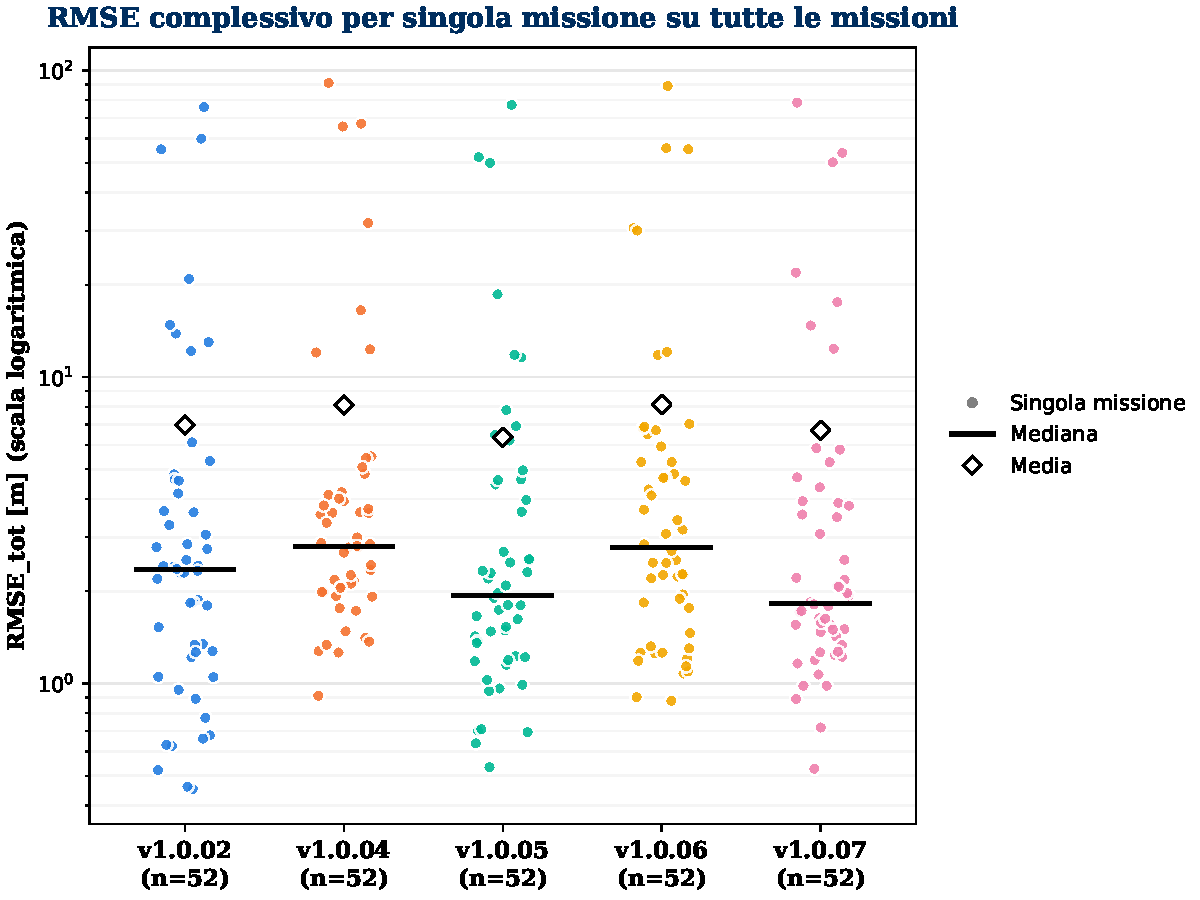
\includegraphics[width=0.49\linewidth]{images/Risultati/variazioni_dati/Strip_plot/RMSE_tot_stripplot_total_missions.pdf}%
                }\\

        \caption{Range plot e scatter plot globali al variare delle features del dataset}
        \label{fig:rp_sp_data}
                
    \end{figure}

I grafici presentati nelle \emph{Figure} \ref{fig:bp_data} e \ref{fig:rp_sp_data}, confermano solo parzialmente le tendenze delineate con l'analisi di correlazione; sebbene la tendenza generale mostri un miglioramento prestazionale con la riduzione della dimensionalità del dataset, la configurazione caratterizzata dall'assenza delle sole componenti verticali si rivela la peggiore in termini di puro valore medio e mediano dell'RMSE, nonostante sia quella che presenta la minore dispersione dell'errore e, pertanto, legata alla maggiore affidabilità della previsione. Come anticipato nella descrizione delle versioni, anche la v1.0.06 risulta essere inadeguata, con prestazioni paragonabili alla v1.0.04 appena citata. Il confronto tra le restanti è, invece, più complesso; la v1.0.05, infatti, presenta il minimo valor medio di RMSE, con una mediana solo leggermente più alta rispetto a quella registrata per la v1.0.07. Tuttavia, quest'ultima è caratterizzata da una distribuzione dell'errore notevolmente più contenuta intorno alla mediana stessa. Considerando, poi, l'impatto delle poche missioni critiche su tutti i valori registrati, si sceglie di procedere con la configurazione corrispondente alla v1.0.07 che, nonostante sembri meno robusta garantisce una maggiore accuratezza della stima nel caso tipico. Nel seguito, per coerenza di forma con il resto dei codici associati alle versioni ci si riferirà a questa con la denominazione \textbf{v1.1.0}.

% Valutare se mettere qui il confronto con il paper o farlo solo nel confronto finale
%Selezionata, quindi, la versione di riferimento per il prosieguo dell'analisi, occorre valutare come 


\section{Analisi al variare della loss function}

Nonostante la rete neurale nella sua prima versione mostri prestazioni già sufficientemente valide, sono ancora presenti possibili margini di miglioramento. Per esplorare meglio queste potenzialità, il primo elemento su cui ci si focalizza è la loss function, responsabile di una buona parte del processo di apprendimento e, di conseguenza, della capacità di generalizzazione e predizione del modello. Nello specifico, come già discusso nel Capitolo 2, la L2 Loss presenta alcune criticità, la più significativa delle quali è legata alla gestione degli outlier nei dati. Una prima variazione può, dunque, comportare proprio la sostituzione di tale funzione con una L1 Loss che, in presenza di effettivi outlier non correttamente gestiti dalla rete neurale, dovrebbe portare ad un miglioramento delle prestazioni del modello. Una soluzione alternativa, decisamente più sofisticata, riguarda, invece, l'utilizzo di una Log-Cosh Loss; come già evidenziato, infatti, una simile funzione consente di ottenere un comportamento più bilanciato, sfruttando i pregi di entrambe le precedenti funzioni. 

In tutti questi casi, tuttavia, vengono sfruttate unicamente le informazioni legate alla differenza tra la posizione target e quella stimata dal modello per ogni secondo di iterazione. Teoricamente, introdurre nel processo anche indicazioni sulla stima della posizione tramite tecniche di dead-reckoning e una maggiore conoscenza dell'evoluzione temporale dell'errore, potrebbe portare degli effettivi benefici prestazionali. Prendendo ispirazione dal lavoro svolto da Wei e Sun\cite{Lp_Wei}, si è, quindi, definita una funzione di perdita originale, basata sull'utilizzo di una \textit{Mixed $L_p$ Norm Regularization}, introdotta per la prima volta da Fournier e Oldenburg\cite{Lp_norm_reg}; pertanto, la funzione sarà identificata proprio con il nome di \textbf{$L_p$ Norm Loss} nel prosieguo. Entrando nel merito, l'approccio proposto dai due autori è stato pensato per poter contemporaneamente stimare i valori di due proprietà geofisiche normalmente associate a modelli differenti, nello specifico la densità ($m_{1}$) e la suscettività ($m_{2}$), a partire da due set di dati distinti. Di conseguenza, la formulazione matematica impiegata tiene conto di questa suddivisione, presentando per ogni modello un termine di errore $\Phi_{d, i}$, di carattere più tradizionale e legato all'errore della previsione $d^{\text{pre}}$ rispetto all'effettivo valore osservato $d^{\text{obs}}$, e un termine di regolarizzazione $\Phi_{m, i}$, calcolato proprio mediante la $L_p$ Norm Regularization, che sfrutta la somma di una componente di \textit{smallness} e una di \textit{smoothness}; a questi si aggiunge, poi, un termine di accoppiamento $\Phi_{c}$, che consente lo scambio di informazioni tra i due modelli ed è basato sul \textit{cross-gradients coupling method}, presentato da Gallardo e Meju\cite{Cross_coupling_gradient}. Il vantaggio principale di un simile approccio consiste nella sua elevata flessibilità, conferita sia dalla possibilità di utilizzare differenti norme per le due componenti del termine di regolarizzazione, sia dall'uso dei numerosi coefficienti presenti nelle relazioni.  

    \begin{equation}
        \begin{aligned}
            \Phi = \Phi_{d,1}(m_{1}) + \Phi_{d, 2}(m_{2}) + \beta_{1} \, \Phi_{m, 1}(m_{1}) + \beta_{2} \, \Phi_{m, 2}(m_{2}) + \lambda \, \Phi_{c} (m_{1}, m_{2}) \\[0.25cm]
            \text{con} \, \, \, \begin{cases}
                \Phi_{d, i} = || w_{d, i} \, (d^{\text{obs}}_{i} - d^{\text{pre}}_{i}) ||_{2}^{2} \\[0.25cm]
                \Phi_{m, i} = \alpha_{s, i} \, || w_{s, i} \, m_{i} ||_{p}^{p} + \sum_{j = x,y,z} \alpha_{j, i} || w_{j, i} \, m_{i} ||_{q}^{q}
            \end{cases}
        \end{aligned}
        \label{eq:Lp_og}
    \end{equation}

Tuttavia, nella rete neurale sviluppata per questa tesi si ha un unico modello, necessario a stimare il vettore degli spostamenti, così come unico è anche il dataset. Tenendo conto di ciò e considerando le specifiche peculiarità legate ad un problema di posizionamento, occorre, dunque, adattare la formulazione mostrata in (\ref{eq:Lp_og}). Nel dettaglio, mentre il termine $\Phi_{d}$ resta pressoché invariato e, sostanzialmente, coincidente con una normale L2 Loss, cambia a livello concettuale il termine di regolarizzazione. In questo caso, infatti, la componente di smallness diventa rappresentativa della distanza tra lo spostamento predetto dalla rete neurale e quello ottenuto tramite integrazione del vettore velocità, mentre quella di smoothness è legata alla differenza tra lo spostamento stimato in secondi consecutivi. Inoltre, si sceglie di introdurre un termine aggiuntivo, legato all'MSE dell'errore complessivamente accumulato nella finestra di osservazione di $K$ secondi. Per quanto detto, la minimizzazione della funzione di perdita passa, di conseguenza, anche dalla riduzione dell'errore rispetto alla navigazione in dead-reckoning, richiamando in parte il meccanismo di funzionamento dell'architettura RBFNN presentata nel Capitolo 3, dal mantenimento di una gradualità nella variazione dello spostamento, favorendo una maggiore attinenza alla dinamica reale, e dalla minimizzazione dell'errore accumulato nei secondi di osservazione di una specifica finestra temporale. Un tema da evidenziare è legato al cambiamento strutturale apportato al meccanismo di suddivisione del dataset, reso necessario proprio dalla presenza del termine $\Phi_{\text{cum}}$. Dovendo valutare l'evoluzione della posizione attraverso più secondi consecutivi, segmentare il dataset in finestre da 1 singolo secondo, ognuna contenente 5 o 10 misurazioni a seconda della frequenza del sensore, aggregate poi in batch da 32 secondi non è più sufficiente. Pertanto, si introduce un ulteriore parametro da ottimizzare in concomitanza del batch size $B$, ovvero la window size $K$. 

Quanto discusso, tenendo conto della necessità di utilizzare termini di spostamento normalizzati, si traduce, a livello matematico, nella formulazione presentata nel seguito, in grado di stimare la loss function per ogni finestra temporale di $K$ secondi considerata in un batch:

    \begin{equation}
        \begin{aligned}
            \Phi = \Phi_{d}(y, \hat{y}) + \alpha_{s} \, \Phi_{s}(\hat{y}, v_{\text{DVL}}) + \alpha_{t} \, \Phi_{t}(\hat{y}, t) + w_{\text{cum}} \, \Phi_{\text{cum}}(\tilde{\hat{\mathbf{y}}}, \tilde{\mathbf{y}}) \\[0.25cm]
            \text{con} \, \, \, \begin{cases}
                \Phi_{d} = \displaystyle || y_{i} - \hat{y}_{i} ||_{2}^{2} \\[0.35cm]
                \Phi_{s} = \displaystyle \frac{1}{K}\sum_{k=1}^{K}\left\|\hat{\mathbf{y}}_{k}-\mathbf{v}_{k}\right\|_{p}^{p} \\[0.35cm]
                \Phi_{t} = \displaystyle \frac{1}{K-1}\sum_{k=2}^{K}\left\|\hat{\mathbf{y}}_{k}-\hat{\mathbf{y}}_{k-1}\right\|_{q}^{q} \\[0.35cm]
                \Phi_{\text{cum}} = \displaystyle \frac{1}{K}\sum_{k=1}^{K}\left\|\sum_{j=1}^{k}\left(\hat{\mathbf{y}}_{j} - \mathbf{y}_{j}\right)\right\|_{2}^{2}
            \end{cases}
        \end{aligned}
        \label{eq:Lp_norm}
    \end{equation}

La loss function così definita introduce, naturalmente, molteplici parametri ignoti all'interno del modello, alcuni dei quali possono assumere valori appartenenti a range molto ampi; un esempio sono i pesi legati ai termini di regolarizzazione, contenuti nel range $[0.01, 1]$. Definire empiricamente la miglior combinazione di parametri per ogni specifica versione della rete neurale, considerando anche la successiva analisi di variabilità della dimensionalità, pur usando un'ottimizzazione Bayesiana, risulterebbe eccessivamente costoso in termini di tempo. Pertanto, in questa trattazione si sceglie di definire specifici valori sulla base del significato fisico e matematico dei vari termini. Si assegna, infatti, maggiore importanza all'errore di deriva accumulato nel corso del tempo, con un peso relativo pari a $w_{\text{cum}} = 0.1$, rispetto ai termini di regolarizzazione, considerati entrambi con un peso di $\alpha_{s} = \alpha_{t} = 0.05$. Per quanto concerne le norme su cui sono basati i due termini di smallness e smoothness, invece, si sceglie di mantenere un valore $p = q = 1$. Se per la prima componente la selezione risulta quasi obbligata, essendo 1 il minimo valore in grado di garantire la convessità della funzione favorendo allo stesso tempo soluzioni sparse, per la seconda la scelta è stata fatta in funzione delle quasi inevitabili brusche variazioni di spostamento presenti, associate a cambi di direzione o manovre specifiche; una norma L2, porterebbe, infatti, a un'eccessiva penalizzazione di questi casi, incrementando la gradualità dell'evoluzione degli spostamenti più del necessario e rischiando, di conseguenza, di perdere le informazioni legate ad alcune manovre compiute. Discorso diverso, invece, riguarda la batch size e la window size, valutate con un procedimento analogo a quello già presentato nel precedente paragrafo. 

Nello specifico, le varianti prese in considerazione sono 8, pensate per valutare le prestazione della rete neurale in funzione di 4 differenti dimensioni delle mini-batch utilizzate per la suddivisione dei dati. Nella seguente tabella sono riportate le combinazioni testate e il relativo codice identificativo, mentre nelle \emph{Figure} \ref{fig:bp_v4_batch} e \ref{fig:rp_sp_v4_batch} sono introdotti i grafici risultanti dal processo di addestramento ed esecuzione dei modelli ottenuti:

    \begingroup
        \footnotesize
        \keepXColumns
        \renewcommand{\arraystretch}{1.4}
        \begin{xltabular}{\textwidth}{|>{\centering\arraybackslash}X|>{\centering\arraybackslash}X|>{\centering\arraybackslash}X|>{\centering\arraybackslash}X|>{\centering\arraybackslash}X|>{\centering\arraybackslash}X|}

            \caption{Versioni della rete neurale al variare delle dimensioni della mini-batch}
            \label{tab:v4_batch} \\
            \hline
            \textbf{Codice versione} & \textbf{Window size} & \textbf{Batch size} & \textbf{Codice versione} & \textbf{Window size} & \textbf{Batch size} \\
            \hline
            \endfirsthead

            \multicolumn{6}{|c|}{{Continua dalla pagina precedente}} \\
            \hline
            \textbf{Codice versione} & \textbf{Window size} & \textbf{Batch size} & \textbf{Codice versione} & \textbf{Window size} & \textbf{Batch size} \\
            \hline
            \endhead

            \hline \multicolumn{6}{|r|}{{Continua nella pagina successiva}} \\ \hline
            \endfoot

            \hline \endlastfoot

            v4.0.01 & 16 & 2 & v4.0.02 & 8 & 4 \\* \cline{1-6}
            v4.0.03 & 32 & 4 & v4.0.04 & 16 & 8 \\* \cline{1-6}
            v4.0.05 & 8 & 2 & v4.0.06 & 4 & 4 \\* \cline{1-6}
            v4.0.07 & 16 & 4 & v4.0.08 & 8 & 8 \\ \hline

        \end{xltabular}
    \endgroup

    \begin{figure}[!htb]
        \centering
        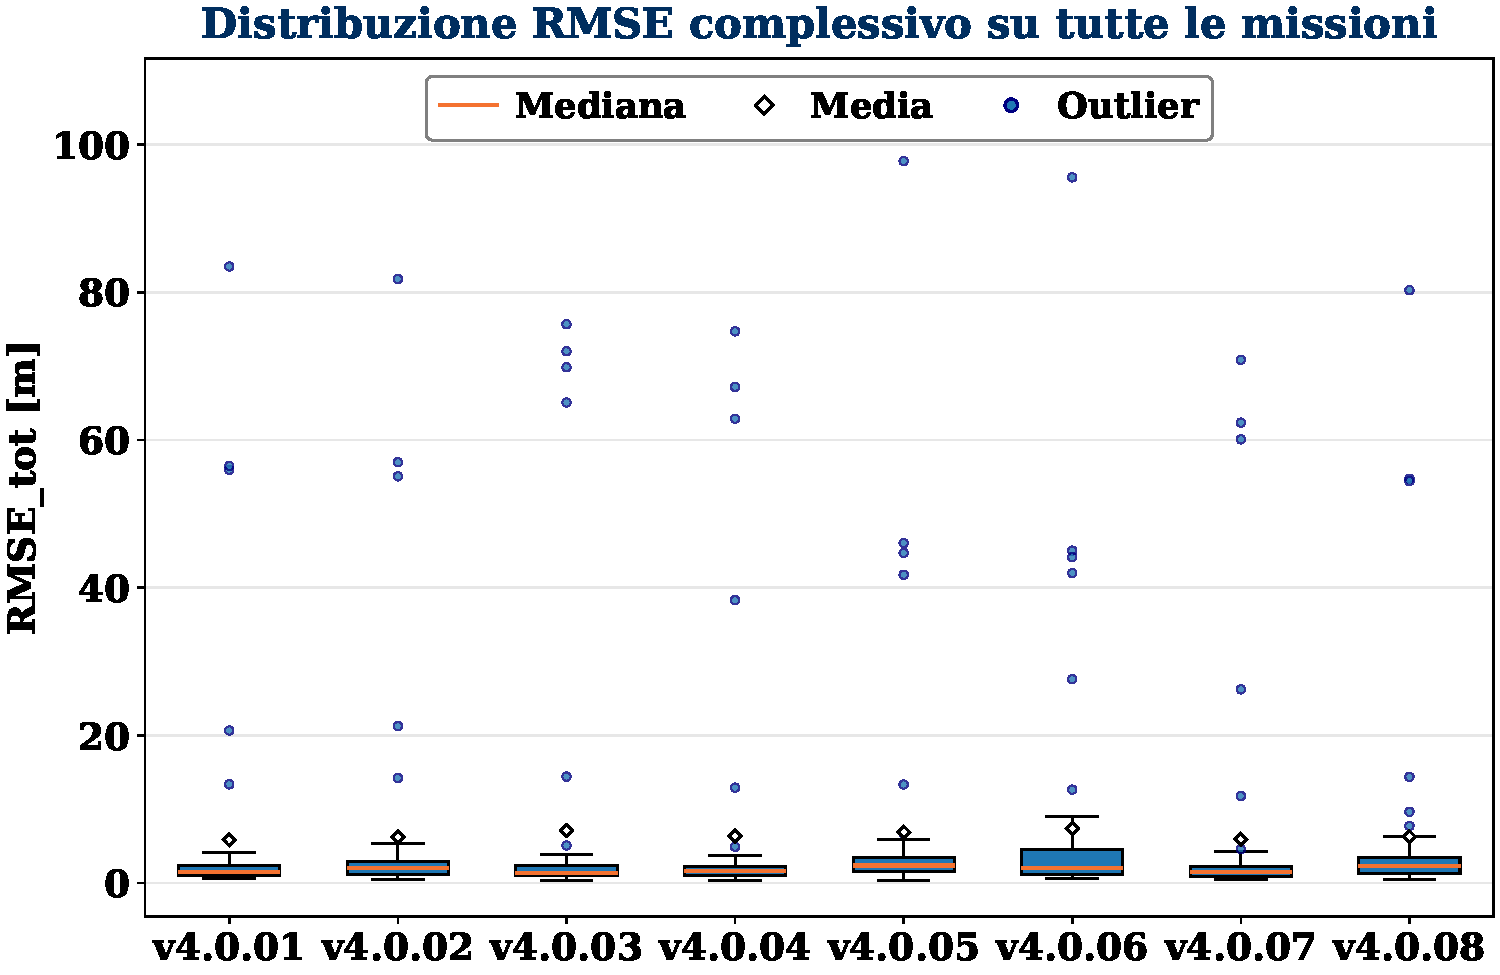
\includegraphics[width=0.8\linewidth]{./images/Risultati/v4/variazioni_windows/Box_plot/RMSE_tot_boxplot_total_missions.pdf}
        \caption{Box plot globale al variare di window e batch size}
        \label{fig:bp_v4_batch}
    \end{figure}

    \begin{figure}[!htb]

        \centering

        \subfloat[Range plot]{%
                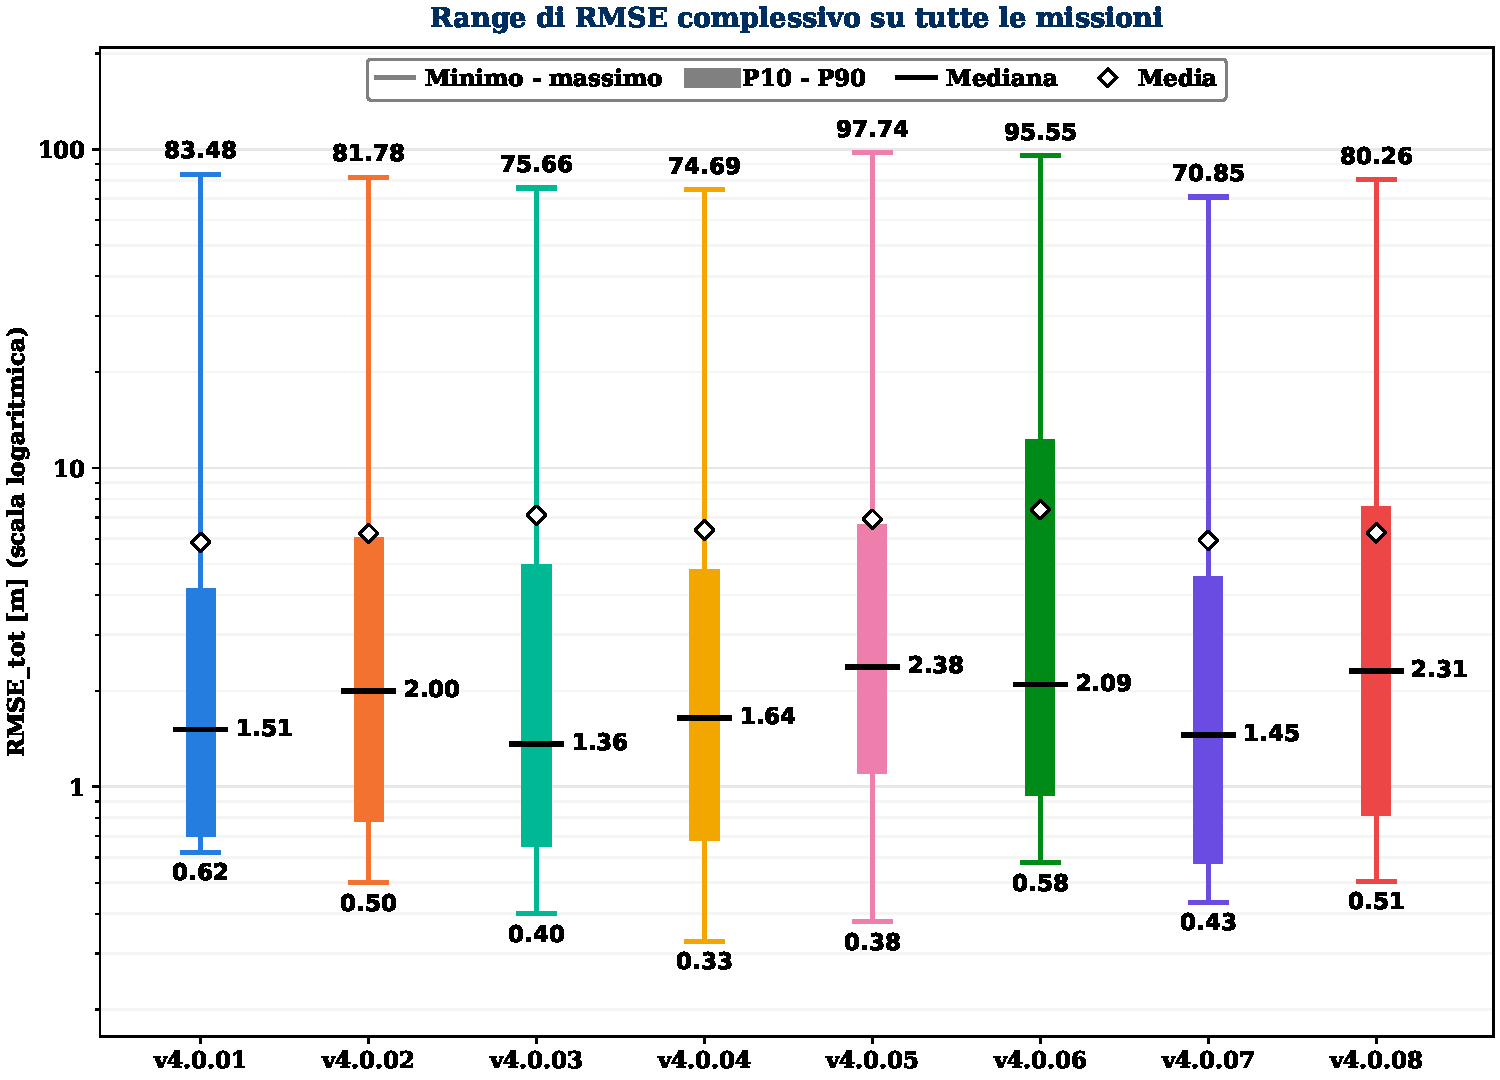
\includegraphics[width=0.50\linewidth]{images/Risultati/v4/variazioni_windows/Range_plot/RMSE_tot_rangeplot_total_missions.pdf}%
                }\hfill
        \subfloat[Scatter plot]{%
                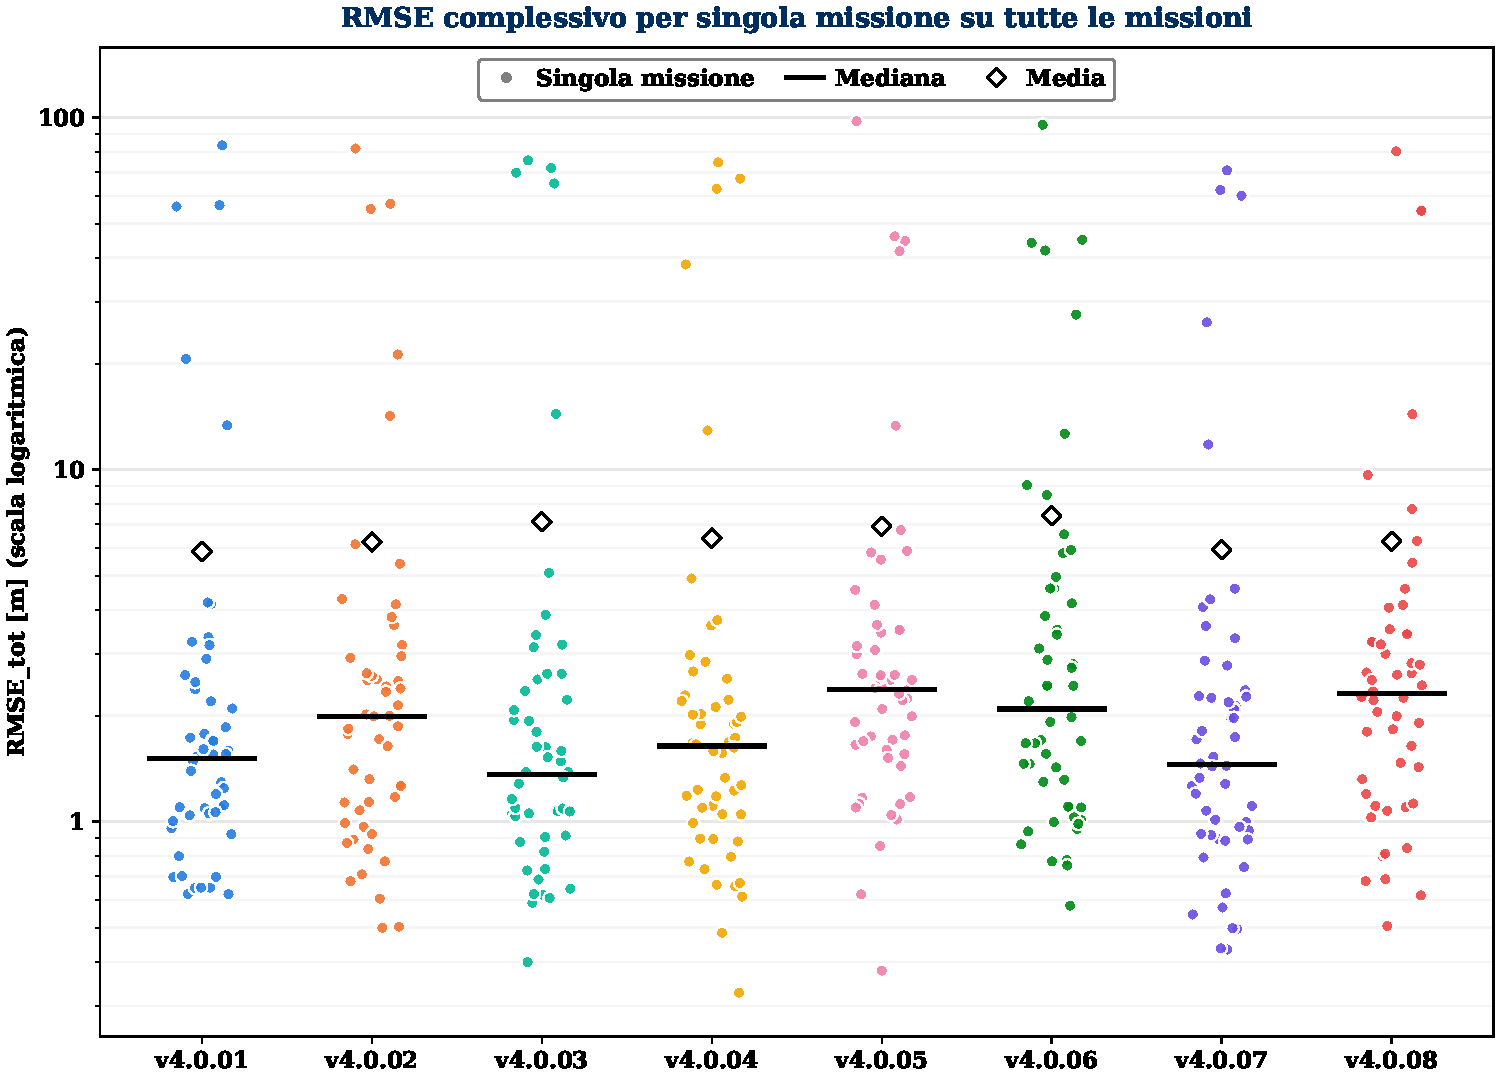
\includegraphics[width=0.49\linewidth]{images/Risultati/v4/variazioni_windows/Strip_plot/RMSE_tot_stripplot_total_missions.pdf}%
                }\\

        \caption{Range plot e scatter plot globali al variare di window e batch size}
        \label{fig:rp_sp_v4_batch}
                
    \end{figure}

Dall'analisi numerica e grafica degli esiti ottenuti, risulta immediatamente possibile scartare le configurazioni associate alla minima dimensionalità considerata, pari a 16 elementi (o secondi) per mini-batch, mentre risaltano le configurazioni v4.0.01, v4.0.03 e v4.0.07. Una prima tendenza osservabile, di carattere più generale, riguarda la distribuzione della dimensionalità; almeno per le combinazioni valutate, infatti, le prestazioni migliori risultano associate alle versioni in cui si dà maggiore spazio ai secondi racchiusi in una singola finestra piuttosto che al numero di finestre prese in esame. Inoltre, per quanto riguarda le tre combinazioni più significative, si evidenzia una sorta di proporzionalità inversa tra media e mediana, con la versione v4.0.01 che presenta allo stesso tempo il minimo valor medio e la più alta mediana, mentre avviene l'opposto con la v4.0.03. In questo senso, pertanto, si individua nella v4.0.07 il miglior bilanciamento tra robustezza e precisione e, di conseguenza, nel seguito questa combinazioni di parametri verrà utilizzata come standard per le versioni basate su questa loss function. 

Valutato anche quest'ultimo aspetto è possibile procedere con la comparazione dei modelli ottenuti sfruttando la struttura base della rete NavNet e le varie funzioni di perdita considerate. I risultati, presentati 

    \begin{figure}[!htb]
        \centering
        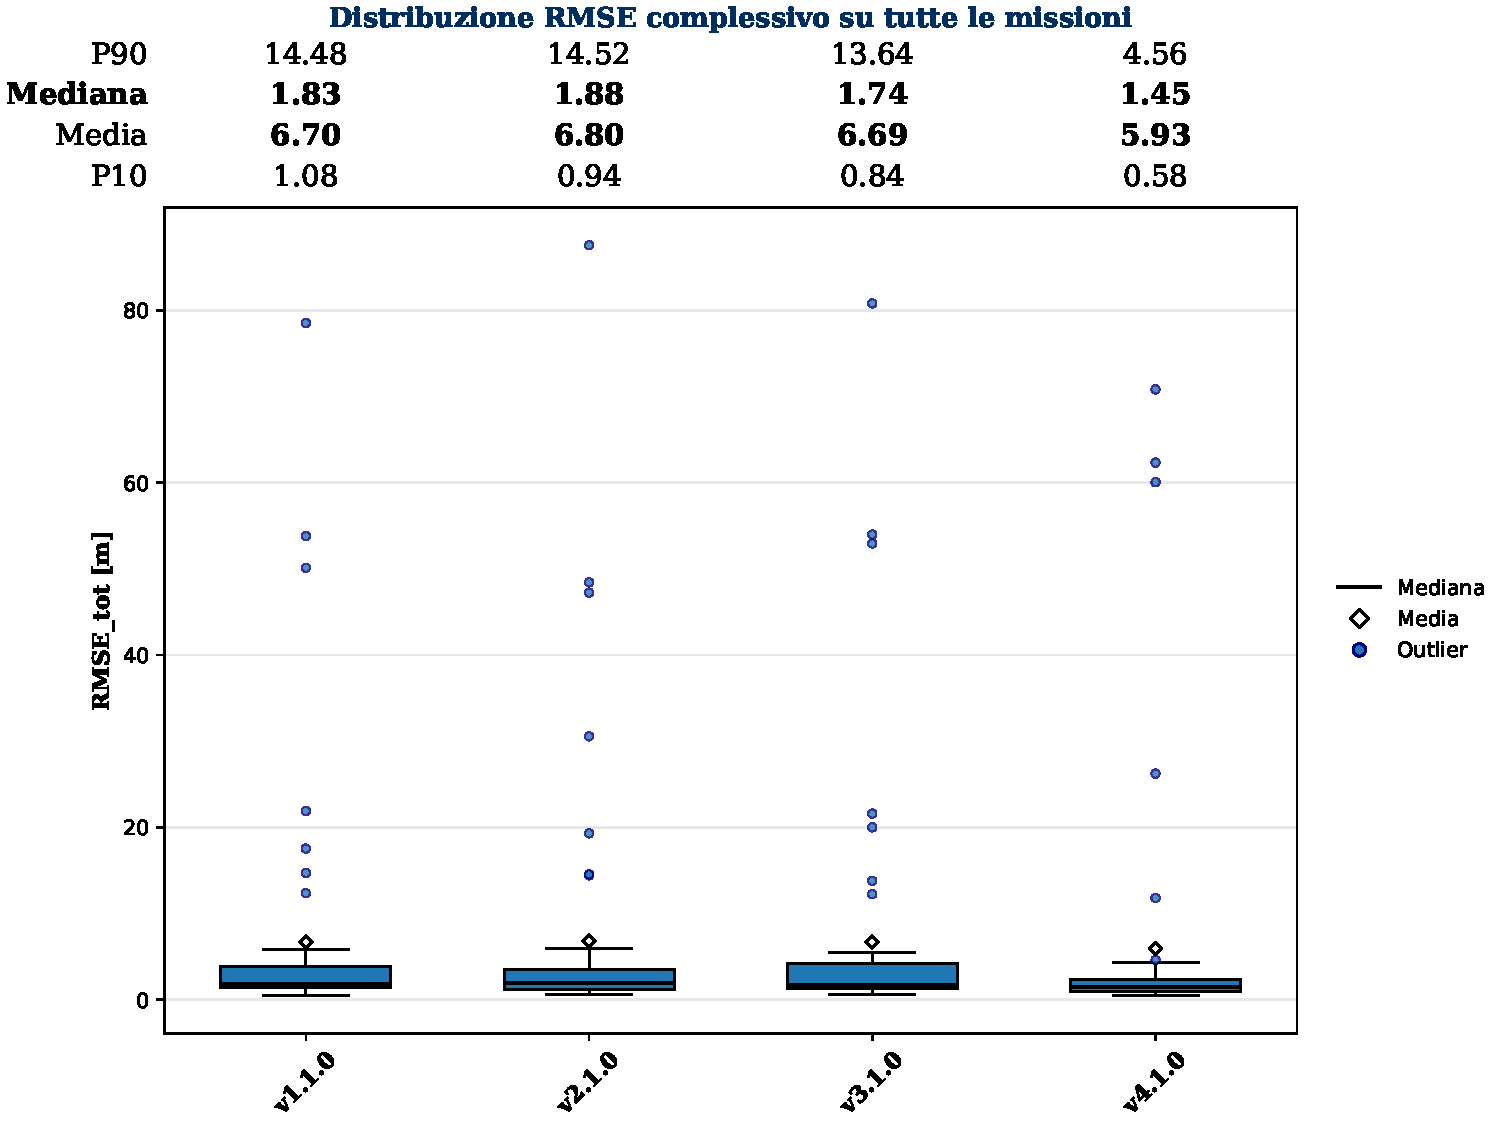
\includegraphics[width=0.8\linewidth]{./images/Risultati/variazione_loss_function/Box_plot/RMSE_tot_boxplot_total_missions.pdf}
        \caption{Box plot globale al variare della loss function}
        \label{fig:bp_loss}
    \end{figure}

    \begin{figure}[!htb]

        \centering

        \subfloat[Range plot]{%
                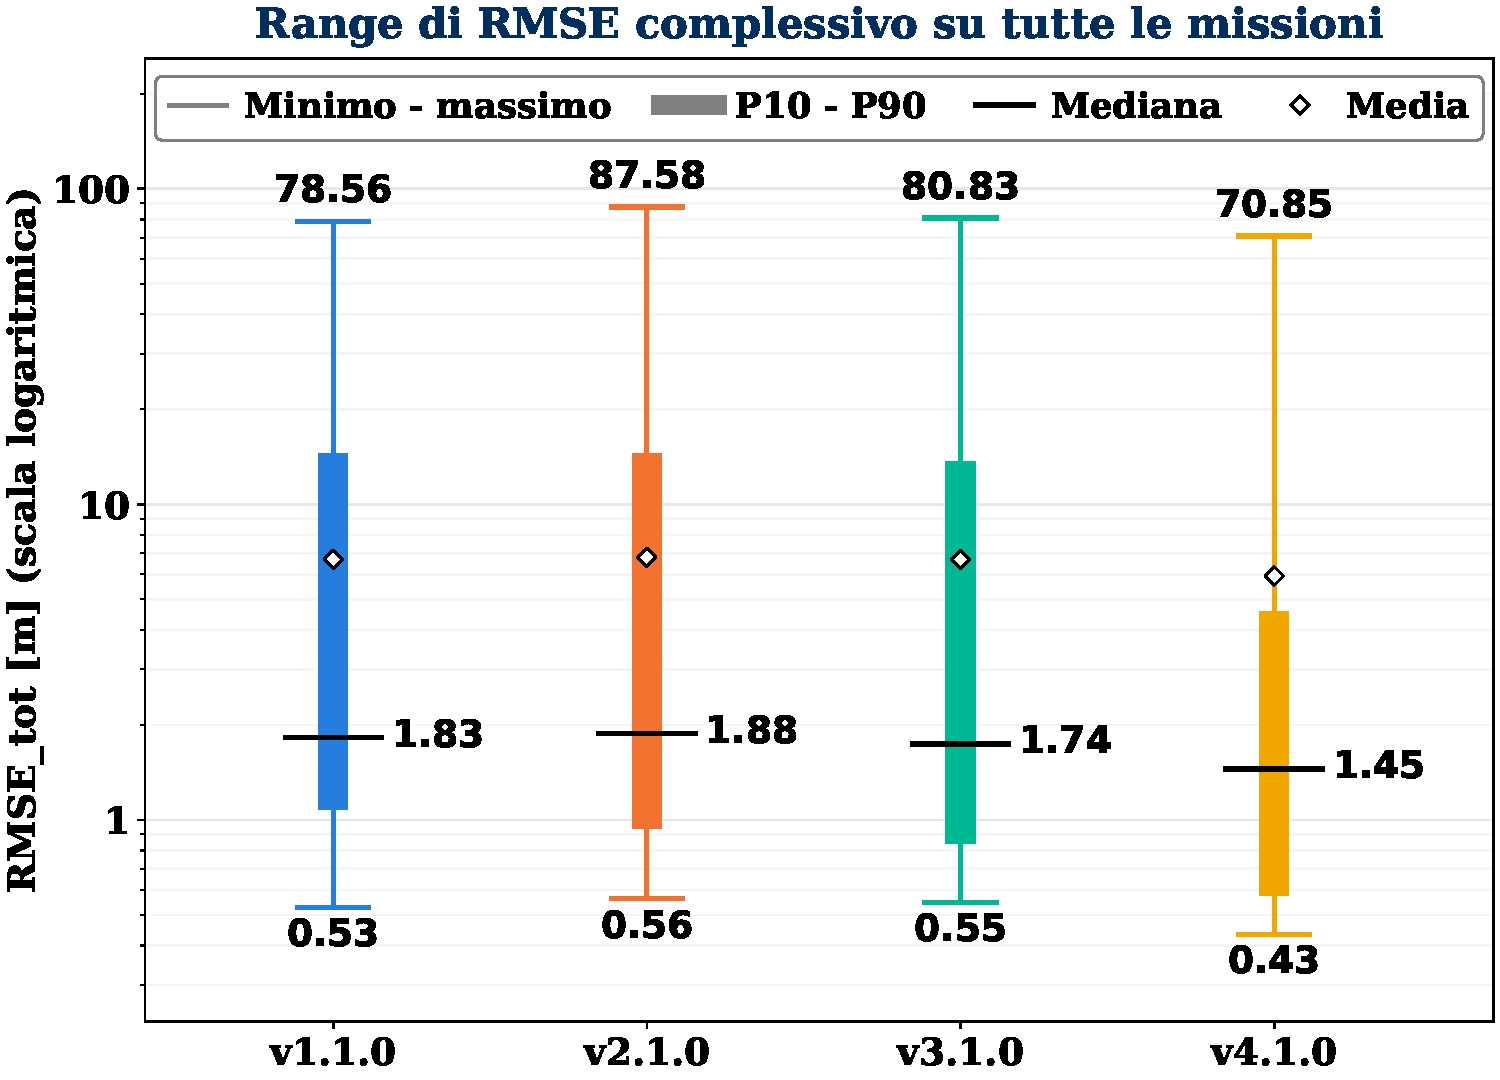
\includegraphics[width=0.50\linewidth]{images/Risultati/variazione_loss_function/Range_plot/RMSE_tot_rangeplot_total_missions.pdf}%
                }\hfill
        \subfloat[Scatter plot]{%
                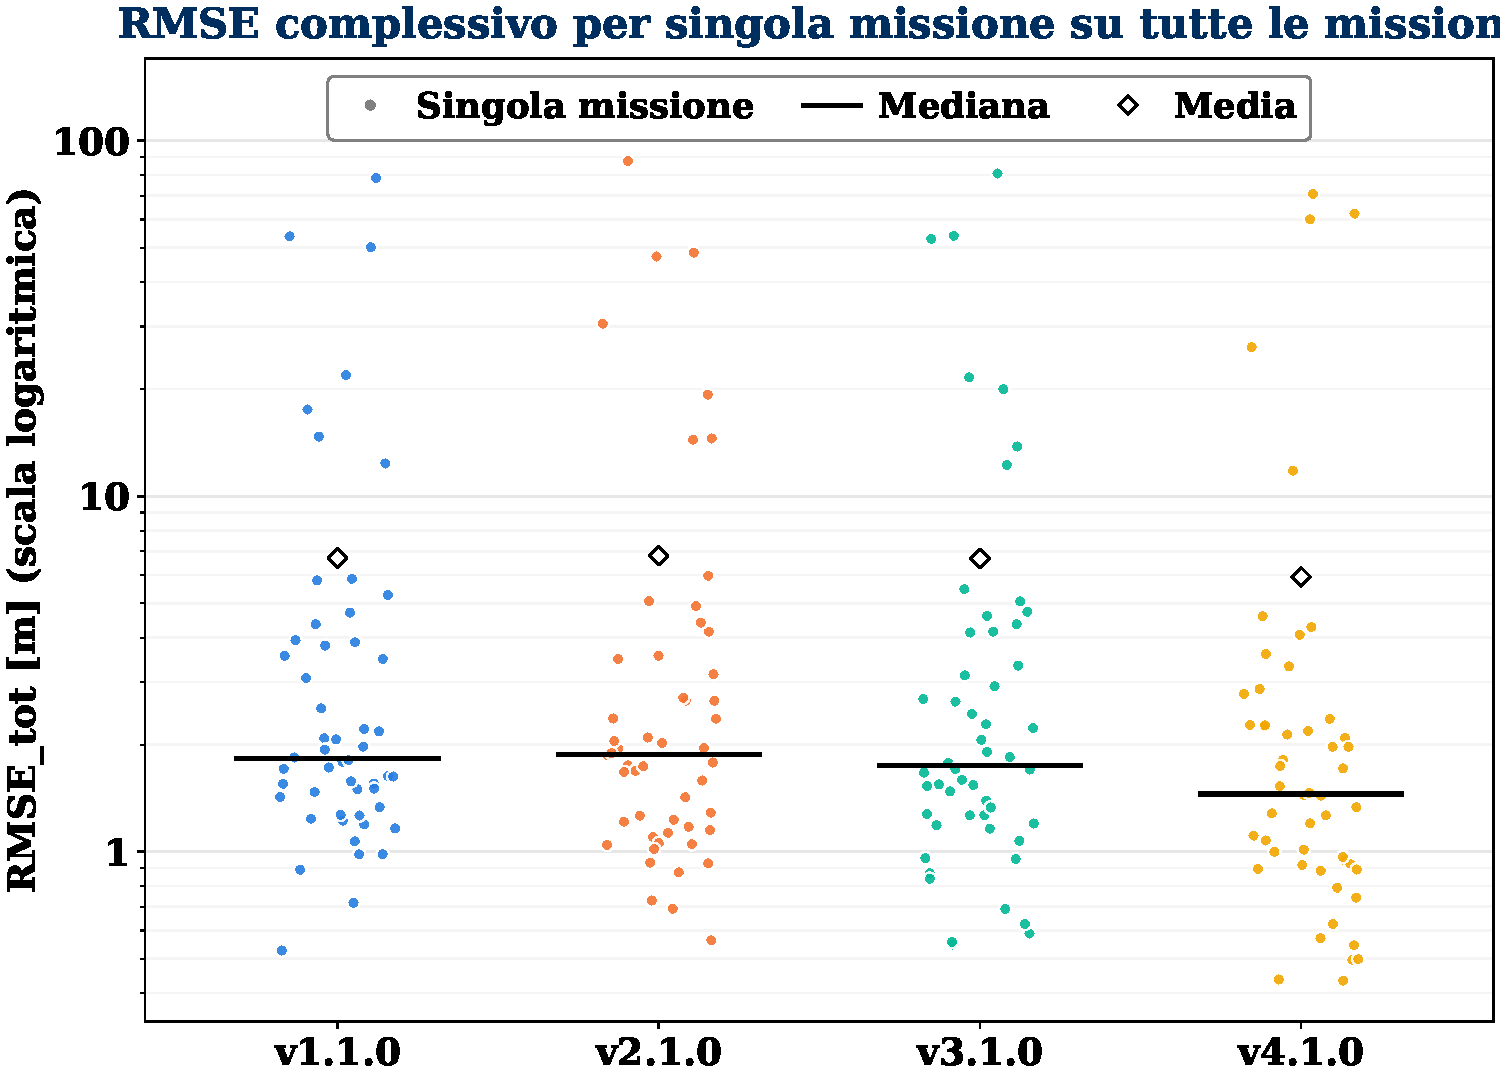
\includegraphics[width=0.49\linewidth]{images/Risultati/variazione_loss_function/Strip_plot/RMSE_tot_stripplot_total_missions.pdf}%
                }\\

        \caption{Range plot e scatter plot globali al variare della loss function}
        \label{fig:rp_sp_v4_loss}
                
    \end{figure}














Per quanto detto, è stato effettuato un addestramento del modello basato su ognuna delle quattro loss function. I risultati sono presentati nel seguito:

% Inserire il grafico con le 4 versioni base considerate


\section{Analisi al variare della dimensionalità}

\subsection{Variazioni della hidden size}

\subsection{Variazioni del numero di fully connected layers}

\subsection{Variazioni combinate}






% QUesto è da indicare indirettamente mettendo i risultati a fianco di una tabella dettagliata riassuntiva della struttura base
%Per quanto riguarda le traiettorie del paper, in particolare, sono forniti i seguenti errori medi sulla posizione: 

\small
\renewcommand{\arraystretch}{1.10}       % Riduce l'altezza delle righe 
\setlength{\LTpre}{8pt}                  % Riduce lo spazio prima della longtable
\setlength{\LTpost}{6pt}                 % Riduce lo spazio dopo della longtable
\setlength{\belowcaptionskip}{5pt}       % Riduce lo spazio sotto la didascalia
\begin{longtable}{ccc}

            \caption{Valori dell'errore in termini di RMSE medio e posizione finale} 
            \label{tab:errori_paper} \\
            
            \toprule
            \textbf{ID traiettoria} & \textbf{RMSE [m]} & $\mathbf{\Delta_{pos} [m]}$\\
            \midrule
            \endfirsthead
            
            \toprule
            \textbf{ID traiettoria} & \textbf{RMSE [m]} & $\mathbf{\Delta_{pos} [m]}$ \\
            \midrule
            \endhead

            \midrule
            \multicolumn{3}{r}{{Continua nella pagina successiva}} \\
            \endfoot

            \bottomrule
            \endlastfoot

            1 & 1.7984 & 2.7435 \\
            2 & 1.9538 & 0.9324 \\
            3 & 2.1145 & 3.2894 \\
            4 & 2.5404 & 3.5220 \\
    
\end{longtable}

     \begin{figure}[!htb]

        \centering

        \subfloat[Minimo locale]{%
                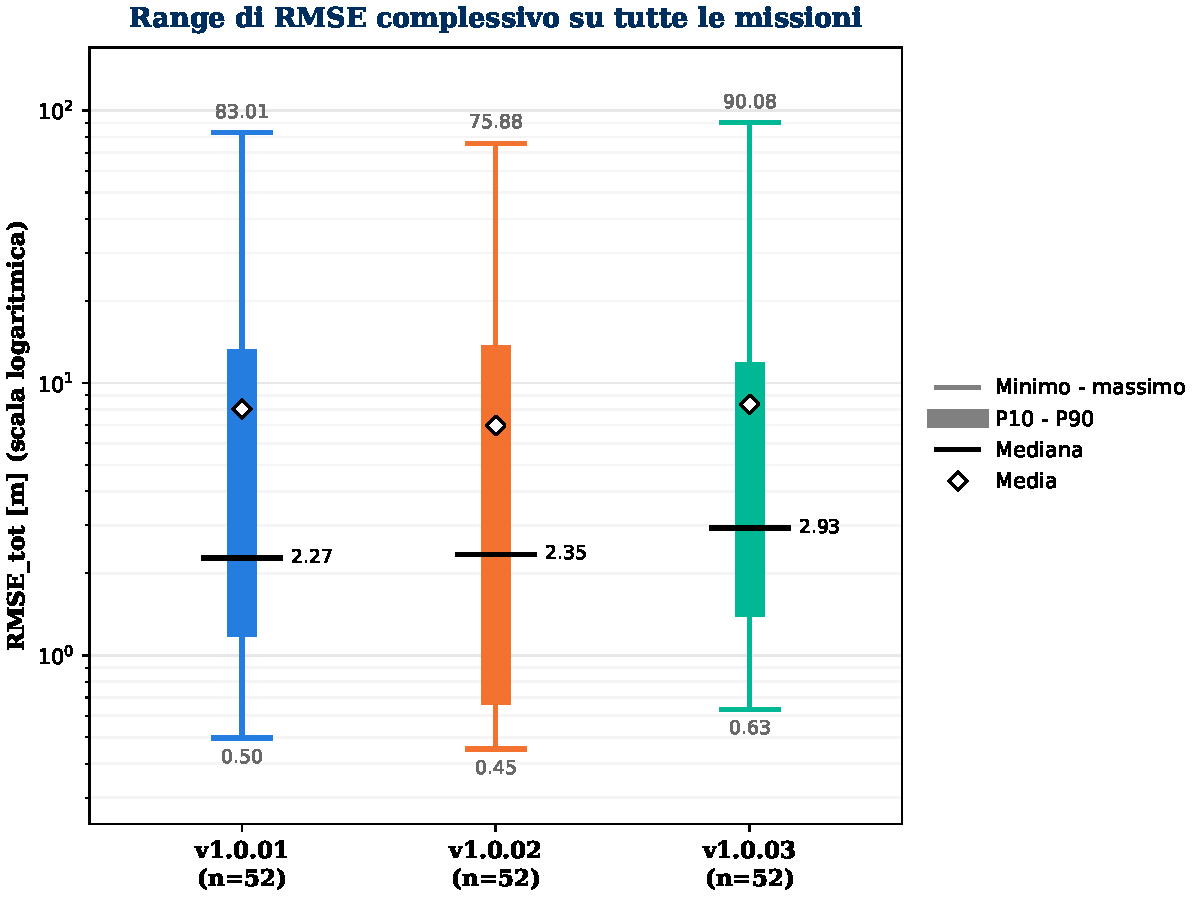
\includegraphics[width=0.50\linewidth]{images/Risultati/variazioni_batch/Range_plot/RMSE_tot_rangeplot_total_missions.pdf}%
                }\hfill
        \subfloat[Massimo locale]{%
                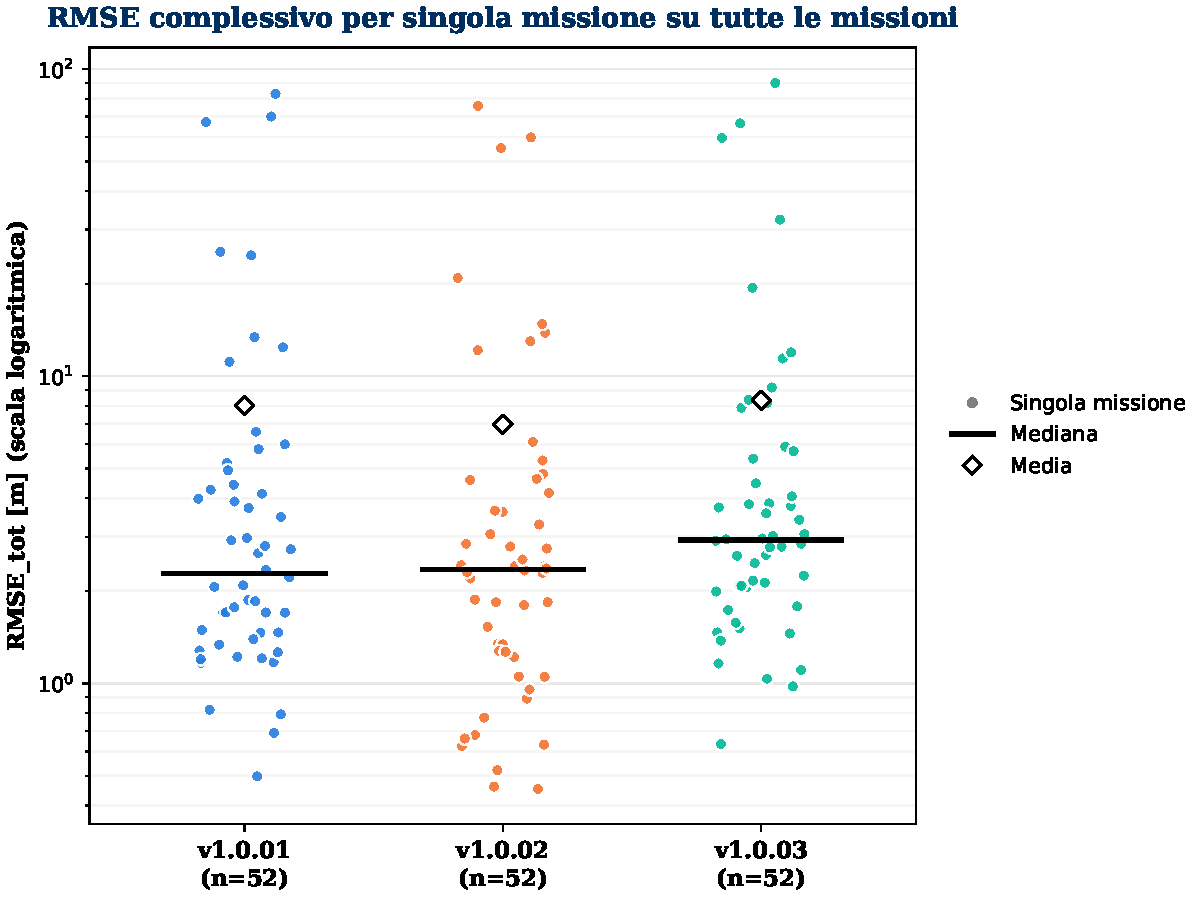
\includegraphics[width=0.49\linewidth]{images/Risultati/variazioni_batch/Strip_plot/RMSE_tot_stripplot_total_missions.pdf}%
                }\\
        \subfloat[Punto di sella]{%
                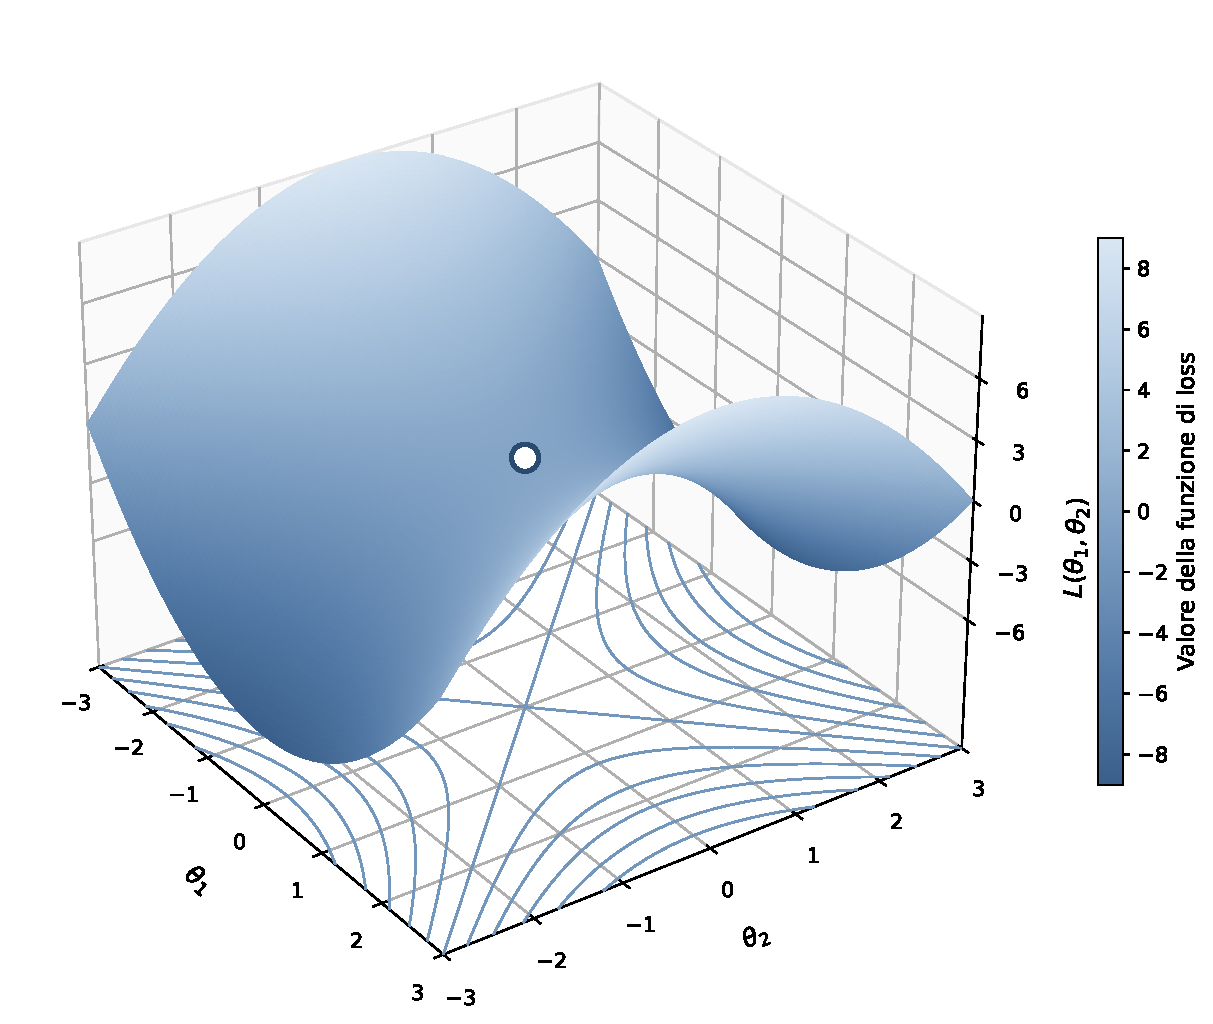
\includegraphics[width=0.33\linewidth]{images/NN/punto_di_sella.pdf}%
                }

        \caption{Range plot e strip plot globali al variare del batch size}
        \label{fig:rp_sp_batch1}
                
    \end{figure}